\documentclass[slidetop, mathserif, dvipsnames]{beamer}

% \mode<presentation>
% {
% 	\usetheme{Warsaw}
% 	\setbeamercovered{transparent}
% }

% \usepackage{caption}
\usepackage{subcaption}
\captionsetup{compatibility=false}

% \usepackage[dvipsnames]{xcolor}

\mode<presentation>{
	\usetheme{Berlin}
	\setbeamercovered{transparent}
	\usefonttheme{professionalfonts}
}

\usepackage{amsmath, amsfonts, amssymb}
\usepackage{mathrsfs,dsfont}

\newcommand{\norm}[1]{\left\|#1\right\|}
\newcommand{\suchthat}{-\hspace{-10pt}\ni\hspace{-10pt}-}


\AtBeginSection[]
{
   \begin{frame}
       \tableofcontents[currentsection]
   \end{frame}
}

\addtobeamertemplate{navigation symbols}{}{%
    \usebeamerfont{footline}%
    \usebeamercolor[fg]{footline}%
    \hspace{1em}%
    \insertframenumber/\inserttotalframenumber
}

%% want to use verbatim: \begin{frame}[fragile]

\title[OTA]{Introdoction to Optimal Transport Assignments for Object Detection}
\author[chy1010]{Chien, Hung-Yu}
\date{\today}

\begin{document}

\begin{frame}
	\titlepage
\end{frame}

\section[Outline]{}
\begin{frame}
	\frametitle{Outlines}
	\tableofcontents
\end{frame}

\section{Introduction: the Motivation of Label Assignments}

\begin{frame}
    \frametitle{Recall}
    Recall the talk on last Friday, YOLOX proposed by Megvii has the following features:
    \begin{enumerate}
        \item multiple image size input
        \item decoupled heads
        \item anchor-free
        \item multi-positives
        \item SimOTA (simplified version of Optimal Transport Assignment)
    \end{enumerate}

    \quad

    Today we'll focus on the OTA, optimal transport assignment.

\end{frame}

\begin{frame}
    \frametitle{Motivation}

    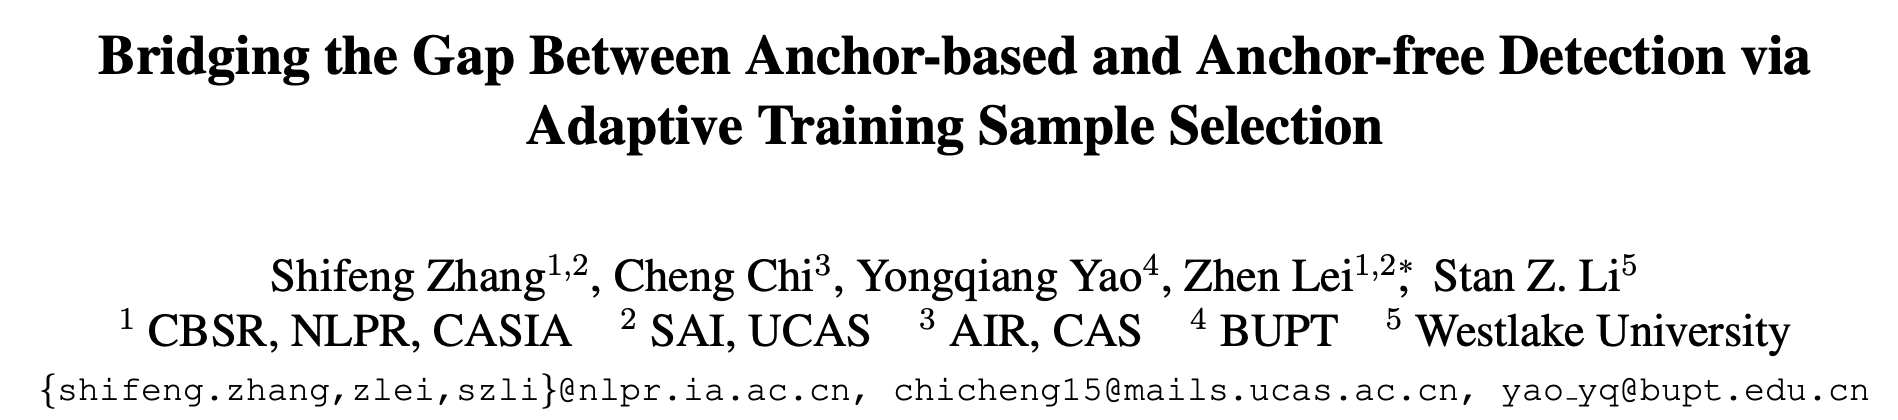
\includegraphics[width=300pt]{pics/atss_paper.png}

    \quad

    In these 2 to 3 years, anchor-free detectors have become popular
    due to the design of FPN and focal loss.
    However, in this CVPR 2020 paper (denoted by ATSS), the authors point out that:
    the {\bf essential difference} between the performance of these proposed
    anchor-based and anchor-free detectors is actually
    {\bf how to define positive and negative trainng samples}.

\end{frame}

\begin{frame}
    \frametitle{Motivation}

    For usual detectors, since it is unknown that how many objects in an image,
    the RPN (region proposal networks) always makes dense predictions at each
    point on the feature map.

    \quad

    While at training, the {\bf imbalance} between ground-truth objects and dense
    sampling of possible object locations has trailed the accuracies.

    \quad

    In 2017, the focal loss is originally designed to address the extreme imbalance
    between {\bf fore- and back-ground classes} during training.
    In particular, the easily classified backgrounds comprise the majority.
    This loss aims to 
    {\bf down-weight these easy samples} and thus
    {\bf focus on training hard samples}.
\end{frame}

\begin{frame}
    \frametitle{Motivation}

    As focal loss try to alleviate the gradients from dominant easy samples,
    the core problem is still to sample training targets from the proposals:
    {\it To train, or not to train, that is the question.}
    \begin{itemize}
        \item positive samples: some object exists in this proposal.
            Need to train the classifier and regressor (anchor's offsets).
        \item negative samples: no object, or belong to the background class.
            Need to train the classifier to output 0 or the background class.
        \item ignore samples: not involed in training process.
    \end{itemize}

    Here we use `label assigment' to mention the association among
    proposals and ground-truth objects in training process.
\end{frame}

\begin{frame}
    \frametitle{Motivation}

    Back to the paper ATSS, they align the anchor-based (RetinaNet)
    and anchor-fre (F-COS) detectors by adding the same tricks:

    \begin{figure}
    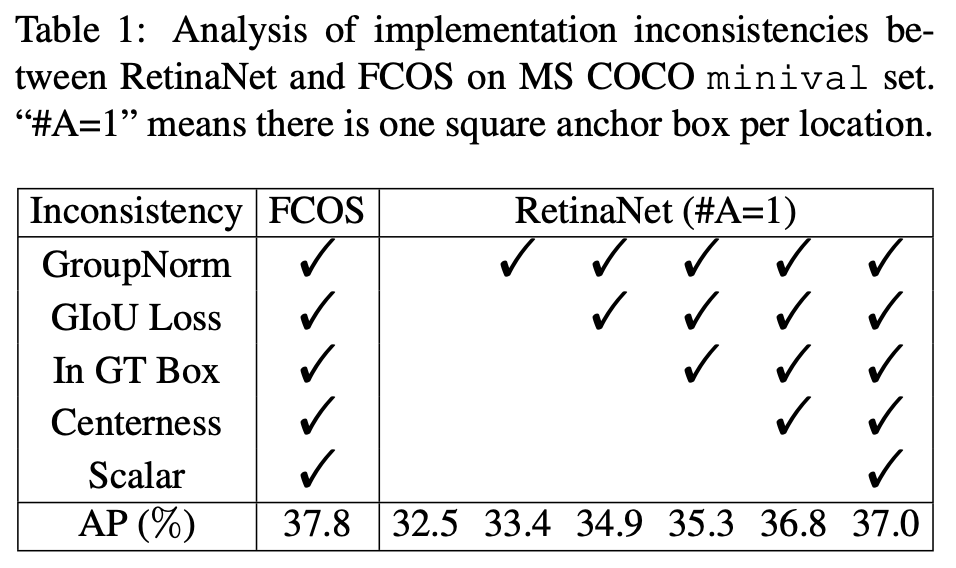
\includegraphics[width=150pt]{pics/atss_compare.png}
    \end{figure}

    Also, on each point of feature map, set $\#A=1$ means
    to use only one single squared box to be an anchor.
    This is aim to compare an anchor point and an anchor box directly.

    % Scalar here means for different feature levels of FPN,
    % the regression values are in fact in different scales.
    % As a result, instead of using the standard exp(x),
    % for the feature level P_i, using exp(s_ix) with a trainable 
    % scalar s_i to automatically adjust the output.

\end{frame}

\begin{frame}
    \frametitle{Motivation}

    Hence the rest differences of their RetinaNet and F-COS are
    \begin{enumerate}
        \item the way to define positive and negative samples: Use IoU threholds (RetinaNet),
            use spatial constraints (F-COS).
        \item the regression starting from an `anchor box` (RetinaNet)
              or an `anchor point` (F-COS).
    \end{enumerate}

    \begin{figure}
    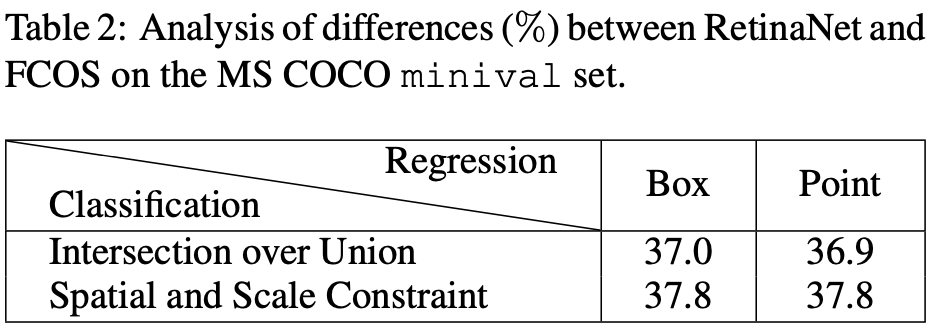
\includegraphics[width=150pt]{pics/atss_compare2.png}
    \end{figure}
    From the table in ATSS, we can see that the main difference
    is the way to define positive and negative samples.

\end{frame}

\begin{frame}
    \frametitle{Motivation}

    The MORAL is that {\bf it is important to choose training targets},
    that is, to re-thinking about how to do the {\bf `label assignments'}.

\end{frame}

\section{Methods to Do Assignments}

\begin{frame}
    \frametitle{Assignments for Anchor-based Detector}

    For anchor-based detectors, the selection of positive and negative samples
    is often determined by the IoU of anchors and ground-truth objects.

    \begin{itemize}
    \item RPN in Faster R-CNN uses $0.7$ and $0.3$ as the thresholds for positive
        and negative samples.
    \item The R-CNN module uses $0.5$ as the pos/neg division.
    \end{itemize}
    This setting is widely used in Faster R-CNN's variants.
    % This kind of label assignments is proved effective and soon been adopted by
    % Faster R-CNN's variants and many one-stage detectors.

    \quad

    Moreover, while the positive samples are still much more than ground truths,
    only a limited number of them are randomly chosen to the calculations of
    gradient descents.

\end{frame}

\begin{frame}
    \frametitle{Assignments for Anchor-free Detector}

    On the other side, anchor-free detectors such as FCOS, Foveabox, and etc.,
    assign positive samples if the location of the anchor point 
    \begin{enumerate}
    \item lies in a ground truth bounding box (F-COS);
    \item or lies in a shrunk version of it (Foveabox, more centralized).
    \end{enumerate}

    \quad

    Furthermore, for another stream of anchor-free models:
    CornerNet, CenterNet, and etc., these models view objects as a point or
    a set of keypoints and hence have distinct characteristics from other
    detectors. We will not discussed this kind of models here.
    
\end{frame}


\begin{frame}
    \frametitle{Dynamic Assignments}

    The label assignment methods mentioned above are determined by fixed thresholds
    or spatial relations among dense predictions and ground truth objects.

    \quad

    Aiming to improve the assigning procedure, many methods are developed
    to produce anchor boxes / anchor points in more fancy ways:
    {\bf GuidedAnchoring}, {\bf MetaAnchor}, {\bf NoisyAnchors},
    {\bf FreeAnchor}, {\bf ATSS}, {\bf PAA}, {\bf AutoAssign} and etc.
    (We just list some of them here.)

    \quad

    FOr example, for every ground truth, {\bf ATSS} select $k$ anchors the most
    close to it. And calculate the {\tt mean} and {\tt std} of IoU's of all
    anchors and objects.
    Then use {\tt mean$+$std} as the new threshold.

\end{frame}

\begin{frame}
    \frametitle{Further Idea for Label Assignment}

    Most of the label assignment methods explore the optimal assigning strategy
    for indivisual ground truth objects. But this failing to
    \underline{consider context information from a global perspective}.

    \quad

    DeTR is the first work that attempts to consider label assignment from
    a global view. By using Hungarian algorithm,
    an optimal bipartite matching between predictions
    and ground truth objects is made and the minimal loss in this iteration
    is obtained.

    \quad

    Why the global perspective is important?
    When the ground truths are crowded, there may be some ambiguous
    anchors which are hard to distribute to ground truth
    objects in the neighborhood.

\end{frame}

\begin{frame}
    \frametitle{Further Idea for Label Assignment}

    \begin{figure}
    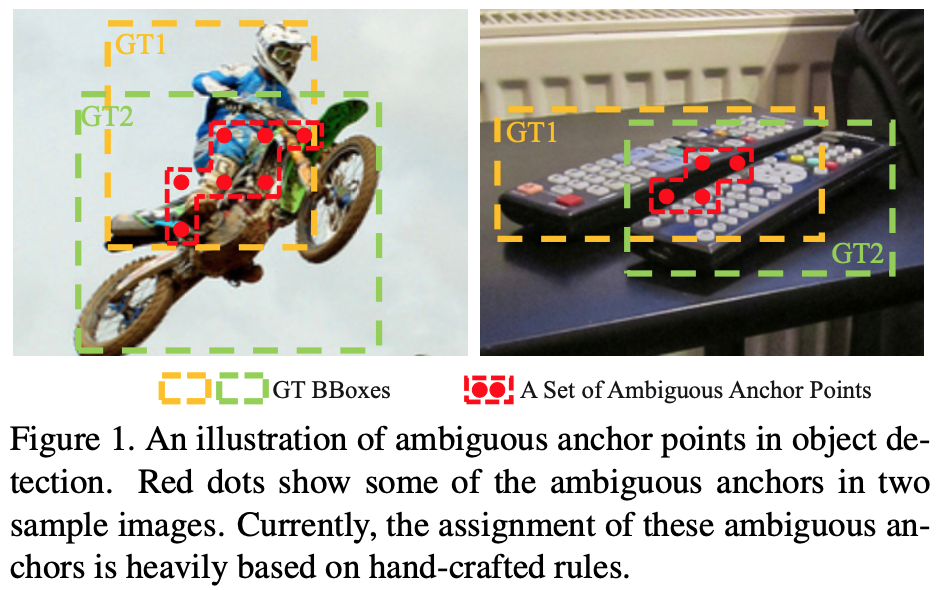
\includegraphics[width=200pt]{pics/ota_motivation.png}
    \end{figure}

    For this anchor-free detector, the anchor points which lie in the
    intersection of two ground truth boxes might be assigned as positive
    samples to only one ground-truth objects.

\end{frame}

\begin{frame}
    \frametitle{Optimal Transport Assignments}

    Unlike DeTR, for CNN-based detectors, the networks often produce
    several regions with high confidence around a ground truth.
    Hence each ground truth object is likely to be assigned mutiple anchors
    to train. And this also helps the \underline{training efficiency}.

    \quad

    Therefore, by extending the idea of using Hungarian algorithm,
    {\bf optimal transport assignment} is proposed
    to achieve the global optimal assignment under
    the {\bf one-to-many situations}.

    \quad 

    Now in a one-to-many manner, we see each gt label as a supplier and each
    anchor a demander.
    Later we will introduce this problem again in an optimal transport's form.

\end{frame}


\section{Optimal Transport Assignment}

\begin{frame}
    \frametitle{What is OT (optimal transport)?}

    Suppose there are $m$ {\it suppliers} and $n$ {\it demanders}.
    The $i$-th supplier holds $s_i$ units of goods and $j$-th demander
    needs $d_j$ units of goods.
    {\it Transporting cost} of each unit of good from $i$-supplier
    to $j$-th demander is denoted by $c_{ij}$.
    The total ammounts are assumed equal: $\sum_{i}s_i = \sum_j d_j$.

    \quad
    
    The goal of this simplest OT problem is to find a {\bf transportation plan}
    $\pi^\star = \{\pi_{ij}\}$ to solve the minimization problem with constraints:
    \[
        \min_\pi\left\{\sum_{i,j} c_{ij}\pi_{ij}\ \left|\ \sum_i \pi_{ij} = d_j,~ \sum_j \pi_{ij}=s_i,
        ~ \pi_{ij}\in\mathbb N\cup\{0\}\right.\right\}.
    \]
    
\end{frame}

\begin{frame}
    \frametitle{A Graph for an Optimal Transport Problem}

    \begin{figure}
    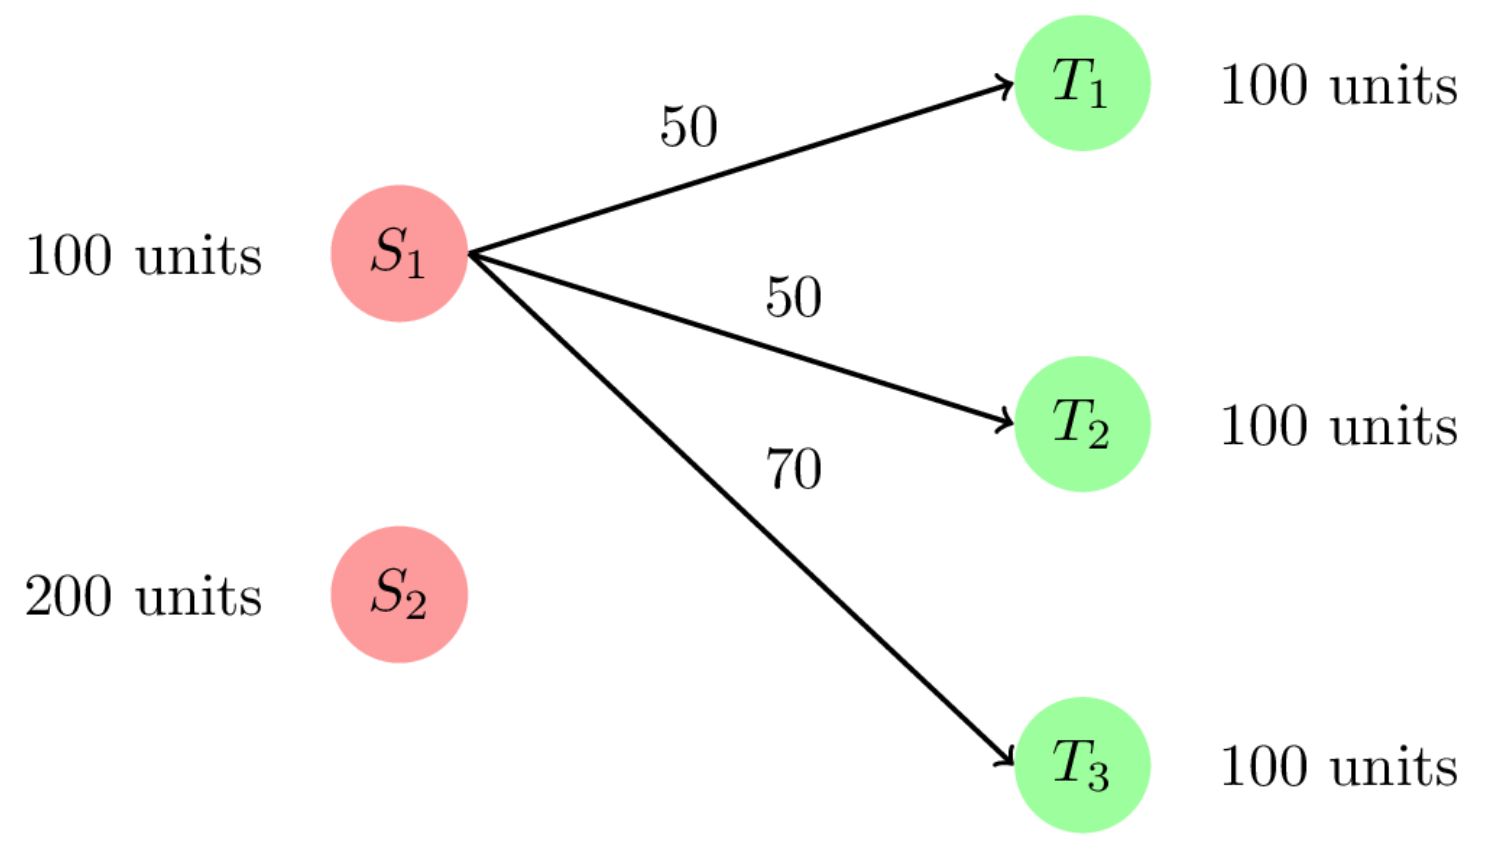
\includegraphics[width=200pt]{pics/ota_graph.png}
    \end{figure}

    In original problem, the unit costs are relative to the distances.
    To our case, the unit costs are defined to be the losses.

\end{frame}

\begin{frame}
    \frametitle{Formulation of the Optimal Transport Problem}

    The transport unit cost from a ground truth $g_i$ to an anchor $a_j$
    is defined as the weighted sum of their classification and regression losses:
    \[
        c_{ij} = \mathcal L_{\rm cls}(a_j^{\rm cls}, g_i^{\rm cls})
        + \alpha \mathcal L_{\rm reg}(a_j^{\rm box}, g_i^{\rm box}).
    \]
    where
    \begin{enumerate}
    \item $\mathcal L_{\rm cls}$: the classification loss, e.g. cross entropy loss, focal loss.
    \item $\mathcal L_{\rm reg}$: the regressive loss, e.g. IoU, GIoU.
    \item $a_j^{\rm cls}$: class confidence / score.
    \item $a_j^{\rm box}$: the corresponding bbox after regressions.
    \item $\alpha$: a balanced coefficient.
    \end{enumerate}
\end{frame}

\begin{frame}
    \frametitle{Formulation of the Optimal Transport Problem}

    We still need to solve the imbalance between fore- and back-grounds.
    We see the {\bf background class} $bg$ as the $m+1$-th supplier, which supplies
    $n-m\cdot k$ goods where $k$ is a dynamic parameter in the training process.

    \quad

    The unit cost to deliver a good from background to an anchor (negative samples)
    is defined as
    \[
        c_{(m+1)~j} = \mathcal L_{\rm cls}(a_j^{\rm cls}, bg).
    \]
    Thus we have a cost matrix $C\in\mathbb R^{(m+1)n}$ with a supplying vector
    $s\in\mathbb R^{m+1}$ and a demanding vector $d\in\mathbb R^n$.
    Aim to solve for an optimal transportation plan $\pi^\star$.

\end{frame}

\begin{frame}
    \frametitle{Sinkhorn-Knopp Iteration}

    For dense sampling of proposals, to solve for an optimal transportation
    induces a large linear programming problem.

    \quad

    To obtain a good result but in a rather fast way,
    we can convert the problem into a {\bf non-linear convex form}
    by adding an entropic regularization term $E$:
    \[
        \min_{\pi} \sum_{ij} \left[c_{ij}\pi_{ij} + \gamma E(\pi_{ij})\right]
    \]
    where $E(x) = x(\log x-1)$ for $x \in [0,1]$.
    The hyper-parameter $\gamma$ is used to control the intensity
    of the regularization.

\end{frame}

\begin{frame}
    \frametitle{Sinkhorn-Knopp Iteration}

    \begin{figure}
        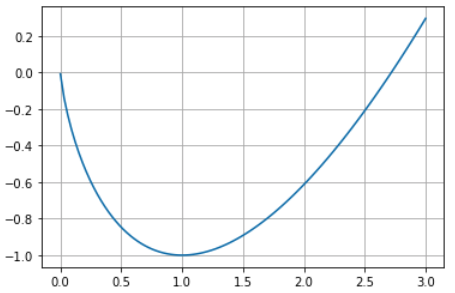
\includegraphics[width=200pt]{pics/ota_entropic_regularization.png}
    \end{figure}

    We can see that $E(x)$ is strictly convex and
    the minimum is at $x=1$.

\end{frame}

\begin{frame}
    \frametitle{Sinkhorn-Knopp Iteration}

    By the Lagrange multiplier method,
    the constrained minimization problem
    \begin{align*}
        \min_{\pi} \Big\{ & \sum_{i,~j} c_{ij}\pi_{ij}+\gamma E(\pi_{ij}) \\
            & + \sum_j \alpha_j\Big(\sum_i \pi_{ij} - d_j\Big)
            + \sum_i \beta_i \Big(\sum_j \pi_{ij} - s_i\Big)
            \Big\}
    \end{align*}
    where $\alpha_j$, $\beta_i$ are the multipliers.
    By letting the derivatives of all parameters equal to 0,
    the optimal plan $\pi^\star$ is resolved as
    \[
        \pi_{ij}^\star =
        e^{-\frac{\alpha_j}{\gamma}}e^{-\frac{c_{ij}}{\gamma}}
        e^{-\frac{\beta_i}{\gamma}}.
    \]

\end{frame}


\begin{frame}
    \frametitle{Sinkhorn-Knopp Iteration}

    Finally we want to obtain the multipliers $\alpha_j$, $\beta_i$
    by solving the constrain equations.

    \quad 

    Denote $u_j = e^{-\alpha_j/\gamma}$, $v_i = e^{-\beta_i/\gamma}$,
    and $M_{ij} = e^{-c_{ij}/\gamma}$.
    By inserting these into the constrain equations:
    \[
        \begin{cases}
        d_j = \sum_i \pi_{ij} = \sum_i u_jM_{ij}v_i = u_j \sum_i M_{ij}v_i; \\
        s_i = \sum_j \pi_{ij} = \sum_j u_jM_{ij}v_i = v_i \sum_j M_{ij}u_j.
        \end{cases}
    \]
    We solve the equations for $u_j$, $v_i$ (and then $\alpha_j$, $\beta_i$)
    by the iterative scheme (which is just the {\bf Sinkhorn-Knopp Iteration}):
    \[
        u_j^{(t+1)} = \dfrac{d_j}{\sum_i M_{ij}v_i^{(t)}},~
        v_j^{(t+1)} = \dfrac{s_i}{\sum_j M_{ij}u_j^{(t)}}.
    \]

\end{frame}

\begin{frame}
    \frametitle{Sinkhorn-Knopp Iteration}

    After enough times of iterations,
    the approximate optimal plan $\pi^\star$
    can be obtained by the final $u$, $v$:
    \[
        \pi^\star = {\rm diag}(v) M {\rm diag}(u),
    \]
    i.e. $\pi_{ij}^\star = v_iM_{ij}u_j$.

    \quad

    In the code, $\gamma$ and the iteration time $T$ are set to be $0.1$ and $50$.

    \quad 

    Once the plan $\pi^\star$ is obtained. We can decode the result and
    assign the anchor to the ground truth which sends the most goods to it.
\end{frame}

\begin{frame}
    \frametitle{Dynamic $k$ Estimation}

    Since each supplier has $k$ units of goods, each ground truth objects are
    likely to be assigned at most $k$ anchors once time.
    It is a good question that how to determine the value of $k$ during the 
    training process.

    \quad

    Like in ATSS to estimate the threshold by statistics of IoUs,
    in OTA's paper, for each ground truth, we can choose top-$q$ predictions
    according to IoU values first.

    \quad 

    Then we sum up the IoU values of these top-$q$ predictions and the ground
    truth. Hence this value is regarded as an estimate of number of possible
    anchors of this ground truth.

\end{frame}

\begin{frame}
    \frametitle{Compare the Results}

    \begin{minipage}{5cm}
    \begin{figure}
        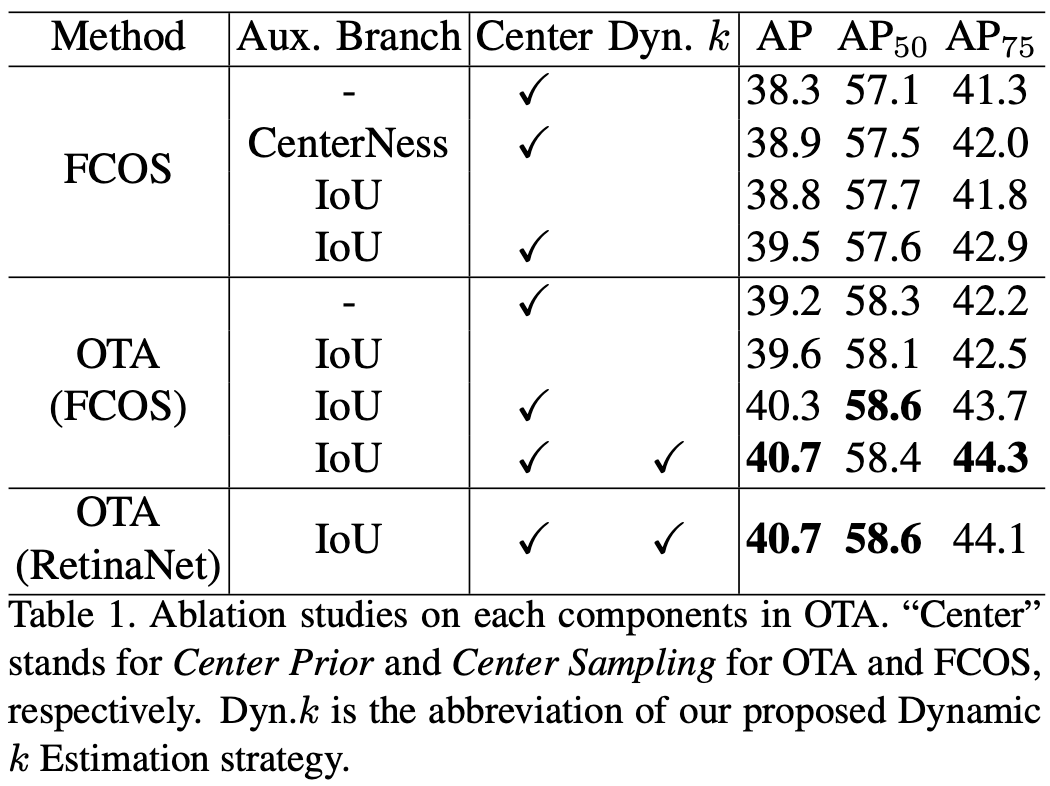
\includegraphics[width=140pt]{pics/ota_compare1.png}
    \end{figure}
    OTA is good.
    \end{minipage}
    \begin{minipage}{5cm}
    \begin{figure}
        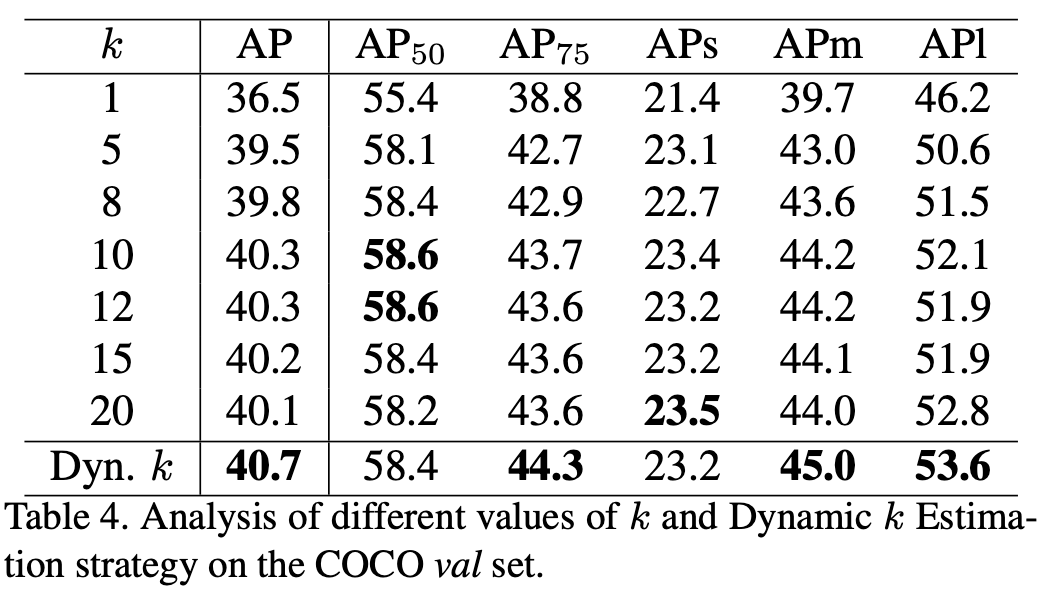
\includegraphics[width=140pt]{pics/ota_compare2.png}
    \end{figure}
    Dynamic $k$ Estimation is good.

    \quad

    \quad

    \end{minipage}

\end{frame}

\begin{frame}
    \frametitle{Thank you AsSign}

    \begin{figure}
        
\includegraphics[width=140pt]{pics/thank-you-road-sign1.jpeg}
    \end{figure}

\end{frame}


\end{document}